% This is the Reed College LaTeX thesis template. Most of the work 
% for the document class was done by Sam Noble (SN), as well as this
% template. Later comments etc. by Ben Salzberg (BTS). Additional
% restructuring and APA support by Jess Youngberg (JY).
% Your comments and suggestions are more than welcome; please email
% them to cus@reed.edu
%
% See http://web.reed.edu/cis/help/latex.html for help. There are a 
% great bunch of help pages there, with notes on
% getting started, bibtex, etc. Go there and read it if you're not
% already familiar with LaTeX.
%
% Any line that starts with a percent symbol is a comment. 
% They won't show up in the document, and are useful for notes 
% to yourself and explaining commands. 
% Commenting also removes a line from the document; 
% very handy for troubleshooting problems. -BTS

% As far as I know, this follows the requirements laid out in 
% the 2002-2003 Senior Handbook. Ask a librarian to check the 
% document before binding. -SN

%%
%% Preamble
%%
% \documentclass{<something>} must begin each LaTeX document
% \providecommand{\main}{..}
\documentclass[../thesis.tex]{subfiles}
% Packages are extensions to the basic LaTeX functions. Whatever you
% want to typeset, there is probably a package out there for it.
% Chemistry (chemtex), screenplays, you name it.
% Check out CTAN to see: http://www.ctan.org/
%%
% \usepackage{graphicx,latexsym} 
% \usepackage{amssymb,amsthm,amsmath}
% \usepackage{longtable,booktabs,setspace} 
% \usepackage{chemarr} %% Useful for one reaction arrow, useless if you're not a chem major
% \usepackage[hyphens]{url}
% \usepackage{rotating}
% \usepackage{hyperref}

% \usepackage{physics}
% \usepackage{siunitx}
% \usepackage{xcolor}

% \usepackage{tikz-feynman}
% \usepackage{standalone}
% \usepackage{natbib}
% Comment out the natbib line above and uncomment the following two lines to use the new 
% biblatex-chicago style, for Chicago A. Also make some changes at the end where the 
% bibliography is included. 
%\usepackage{biblatex-chicago}
%\bibliography{thesis}

% \usepackage{times} % other fonts are available like times, bookman, charter, palatino

\providecommand{\zcut}{z_\mathrm{{cut}}}
\providecommand{\LIPS}{\mathrm{LIPS}}

\providecommand{\cM}{\mathcal{M}}
\providecommand{\cO}{\mathcal{O}}


\setlength{\parskip}{0pt}
%%
%% End Preamble
%%
%% The fun begins:
\begin{document}
	In order to develop an intuition for the mathematical tools we will put to use in the all-orders calculation of groomed heavy hemisphere mass, let us first compute the first-order (or rather, first \textit{nontrivial} order) distribution of the observable. The distribution corresponding to simple electron-positron annihilation with the production of two quark jets, $e^+ e^- \to q\bar q$, would produce a delta function representing a constant measured value: the mass of the heavy hemisphere would simply be half of the final mass. The lowest-order nontrivial distribution corresponds to an $e^+ e^- \to q\bar q g$ event, in which an electron and positron annihilate to produce a quark-antiquark pair, off of which a single gluon is emitted. The location of the gluon in phase space sets the heavy hemisphere mass. This process is depicted in a Feynman diagram in Fig.~\ref{leading-fig:first-order diagram}.

	\begin{figure}[h!]
	\begin{center}
		\begin{tikzpicture}
		\begin{feynman}
			\diagram [horizontal=a to b] {
  				i1 [particle=\(e^{-}\)] -- [fermion] a -- [fermion] i2 [particle=\(e^{+}\)],
  				a -- [photon, edge label=\(\gamma\)] b,
  				f1 [particle=\(\bar q\)] -- [fermion] b -- [fermion] f2 [particle=\(q\)],
			};

			\vertex [above = 0.75cm of f2] (r);
			\vertex [right = 0.1cm of r, label = $g$] (g);
    		\draw [gluon] ($(f2)!0.8!(b)$) -- (r);
		\end{feynman}
		\end{tikzpicture}

		\caption{\label{leading-fig:first-order diagram}Feynman diagram of an $e^+ e^- \to q\bar q g$ event.}
	\end{center}
	\end{figure}

	We will work in the limit that the heavy hemisphere mass $\rho$ is approximately equal to the mMDT cutoff $\zcut$, which is itself small: $\rho \sim \zcut \ll 1$. We will utilize the strategy of regions \cite{becher_introduction_2015-1} to compute the distribution. This is necessary because the distribution is essentially singular in the limit of interest {\color{red}\textbf{[TODO: is this accurate?]}}. The method of regions entails computing the distribution in all singular regions of phase space, then summing the results at the end to generate the full distribution.\footnote{The fact that this works is rather magical.} There are three singular regions of phase space:
	\begin{enumerate}
		\item The \textbf{soft region}, in which the gluon is emitted with low energy.

		\item The \textbf{collinear region}, in which the gluon is emitted collinear to the quark or antiquark.

		\item The \textbf{soft-collinear region}, in which the gluon is both low-energy and collinear to the quark or antiquark. This region is covered by both the soft and the collinear calculations, so we must subtract it away to avoid double-counting.
	\end{enumerate}
	If we label these cross sections $\sigma_\text{soft}$, $\sigma_\text{collinear}$, and $\sigma_\text{soft-collinear}$, respectively, then the full cross distribution will be
	\begin{equation}
		\frac{d\sigma}{d\rho} = \frac{d\sigma_\text{soft}}{d\rho} + \frac{d\sigma_\text{collinear}}{d\rho} - \frac{d\sigma_\text{soft-collinear}}{d\rho}.
	\end{equation}
	Let us calculate these components now.

\section{Soft gluon}
\subsection{Setup}
	For now, we assume a soft (i.e., low-energy) gluon. Recall that the (normalized) heavy hemisphere mass is defined to be
	\begin{equation}
		\rho = \qty(\frac{m_h}{E_h})^2
	\end{equation}
	with $m_h$ the mass of the more massive hemisphere and $E_h$ its energy.

	We first need to sort out the kinematics of the event. Let us shift our reference frame so that the quark has momentum
	\begin{equation}
		p_1^\mu = \frac{Q_q}{2}\qty(1, 0, 0, 1)
	\end{equation}
	and the antiquark has momentum
	\begin{equation}
		p_2^\mu = \frac{Q_q}{2}\qty(1, 0, 0, -1),
	\end{equation}
	and let the gluon have momentum $k^\mu$. The soft-gluon limit means that the energy of the gluon is $k^0 \ll 1$. In this case, the quarks carry most of the energy, so we can approximate $Q_q \approx Q$, the total energy of the event. Furthermore, let us assume that the gluon is emitted in the hemisphere containing the quark (the problem is symmetric under quark-antiquark exchange, so we will simply multiply the cross section by $2$ at the end to account for this assumption). Then the momentum of the heavy hemisphere is
	\begin{equation}
		p_h = p_1 + k,
	\end{equation}
	so the heavy hemisphere has mass
	\begin{equation}
	\begin{aligned}
		m_h^2 &= p_h^2 = \qty(p_{1, 0} + k_0)^2 - (k_1)^2 - (k_2)^2 - (p_{1, 3} + k_3)^2 \\
		&= 2p_{1, 0}k_0 - 2p_{1, 3}k_3 + p_1^2 + k^2 \\
		&= Q(k_0 - k_3).
	\end{aligned}
	\end{equation}
	The last line follows because we assume every particle to be massless, such that $p_1^2 = k^2 = 0$.\footnote{This is a reasonably accurate assumption for the energies accessible by colliders, and makes our calculations much easier. The gluon is actually massless regardless of the theoretical assumptions made.} Now let us introduce the \textbf{light-cone coordinates}
	\begin{align}
		k^+ &\equiv k^0 - k^3 & k^- &\equiv k^0 + k^3,
	\end{align}
	this can be written simply as
	\begin{equation}
		m_h^2 = Q k^+.
	\end{equation}
	The energy of the heavy hemisphere is
	\begin{equation}
		E_h = p_{1, 0} + k_0 = \frac{Q}{2} + k_0 \approx \frac{Q}{2},
	\end{equation}
	since, for a soft gluon, $k_0 \ll Q/2$. The heavy hemisphere mass is therefore
	\begin{equation}\label{leading-eq:soft mass}
		\rho = \frac{Q k^+}{Q^2 / 4} = \frac{4k^+}{Q}.
	\end{equation}
	This means that we will need to insert the measurement function
	\begin{equation}
		\delta\qty(\rho - \frac{4k^+}{Q})
	\end{equation}
	into Fermi's Golden Rule.

	With the kinematics under our belt, let us think about the effects of an mMDT groomer. For the simple case of only 3 particles, the groomer only keeps pairs of particles $i$ and $j$ for which \cite{dasgupta_towards_2013,kardos_two-_2020}
	\begin{equation}
		\frac{\min\qty[E_i, E_j]}{E_i + E_j} > \zcut.
	\end{equation}
	This must be true for the quark and gluon; since the gluon has lower energy then the quark, this necessitates that
	\begin{equation}
		\frac{k_0}{E_h} = \frac{(k^+ + k^-)/2}{Q/2} > \zcut,
	\end{equation}
	or
	\begin{equation}\label{leading-eq:soft grooming}
		k^+ + k^- > Q\,\zcut.
	\end{equation}
	Moreover, since we are assuming that the gluon shares a hemisphere with the quark, we must also have $k_3 > 0$, which requires
	\begin{equation}\label{leading-eq:gluon quark hemisphere}
		k^- - k^+ > 0.
	\end{equation}
	Equations \ref{leading-eq:soft grooming} and \ref{leading-eq:gluon quark hemisphere} generate the phase space constraints
	\begin{equation}
		\Theta\qty(k^+ + k^- - Q\,\zcut)\Theta\qty(k^- - k^+).
	\end{equation}
	When we insert these into Fermi's Golden Rule, the differential cross section takes the form
	\begin{equation}\label{leading-eq:soft cross section preliminary}
		\frac{d\sigma_{\text{soft}}}{d\rho} = 2\int d\LIPS\,\abs{\cM}^2 \delta\qty(\rho - \frac{4k^+}{Q}) \Theta\qty(k^+ + k^- - Q\,\zcut)\Theta\qty(k^- - k^+).
	\end{equation}
	Here, $d\LIPS$ is a differential element of Lorentz-invariant phase space, and $\cM$ is the matrix element governing the $e^+ e^- \to q\bar q g$ process.

	Assuming a soft gluon, the matrix element is well-known in the literature (see Eqs.\ 87 and 88 of \cite{catani_infrared_2000}):
	\begin{equation}
		\abs{\cM}^2 = 4\pi \alpha_s \sigma_0 C_F \mu^{2\epsilon} \frac{p_1 \cdot p_2}{(p_1 \cdot k)(p_2 \cdot k)}.
	\end{equation}
	Here, $\alpha_s$ is the strong coupling constant\footnote{Which is not really a constant.}, $\sigma_0$ is the cross section for $e^+ e^- \to q\bar q$, $C_F$ is the quadratic Casimir of the fundamental representation of color (taken to be $C_F = 4/3$ for our purposes \cite{particle_data_group_review_2020}), and $\mu$ is a mass scale introduced to ensure that the differential cross section will remain dimensionless in $d = 4 - 2\epsilon$ dimensions. Inserting the values of $p_1$, $p_2$, and $k$, we have
	\begin{equation}\label{leading-eq:soft matrix element}
		\abs{\cM}^2 = 4\pi \alpha_s \sigma_0 C_F \mu^{2\epsilon} \frac{2}{k^+ k^-}.
	\end{equation}

	Now we must unpack the Lorentz-invariant phase space element $d\LIPS$. Working in $d$ dimensions, the standard form is
	\begin{equation}
		d\LIPS = \frac{d^d k}{(2\pi)^{d-1}}\delta(k^2)\Theta(k_0),
	\end{equation}
	where the Dirac delta and Heaviside functions ensure that the gluon is on-shell (i.e., real) with positive energy. If $\epsilon = 0$, we would have
	\begin{equation}
		d^d k = d^4 k = dk_0 \,dk_1 \,dk_2 \,dk_3.
	\end{equation}
	When we transform to light-cone coordinates with $(k_0, k_3) \to (k^+, k^-)$, the Jacobian of the transformation is
	\begin{equation}
		\frac{\partial(k_0, k_3)}{\partial(k^+, k^-)} = \mqty(1/2 & 1/2 \\ -1/2 & 1/2),
	\end{equation}
	so
	\begin{equation}
		dk_0 \, dk_3 = \abs{\det \frac{\partial(k_0, k_3)}{\partial(k^+, k^-)}} dk^+ dk^- = \frac{1}{2} dk^+ dk^-.
	\end{equation}
	Now let $k_\perp = (k_1, k_2)$ be the transverse components of the gluon momentum. For $\epsilon \neq 0$, we imagine that these transverse components are the ones which bleed into the modified dimensions. Therefore, after noticing that
	\begin{equation}
		\delta(k^2) = \delta(k_0^2 - k_3^3 - k_\perp^2) = \delta(k^+ k^- - k_\perp^2),
	\end{equation}
	we have
	\begin{equation}
		d\LIPS = \frac{dk^+ dk^- d^{d-2}k_\perp}{2(2\pi)^{d-1}} \delta(k^+ k^- - k_\perp^2)\Theta(k^+ + k^-).
	\end{equation}
	Now it is convenient to transfer the $2 - 2\epsilon$ dimensions of $k_\perp$ into spherical coordinates, so that
	\begin{equation}
		d^{d - 2}k_\perp = k_\perp^{d-3} dk_\perp d\Omega_{d-2}
	\end{equation}
	with $\Omega_{d-2}$ the solid angle of the $(d-2)$-dimensional unit sphere. Since none of the terms in the cross section of Eq.~\ref{leading-eq:soft cross section preliminary} or matrix element of Eq.~\ref{leading-eq:soft matrix element} have angular dependence, we can go ahead and integrate the solid angle:
	\begin{equation}
		\int d\Omega_{d-2} = \frac{2\pi^{(d-2)/2}}{\Gamma(\frac{d-2}{2})}
	\end{equation}
	with $\Gamma(x)$ the gamma function; this identity comes from Eq.\ B.28 of \cite{schwartz_quantum_2014}.
	Therefore,
	\begin{equation}
		d\LIPS = \frac{2\pi^{(d-2)/2}}{\Gamma(\frac{d-2}{2})} \frac{dk^+ dk^- dk_\perp}{2(2\pi)^{d-1}} k_\perp^{d-3} \delta(k^+ k^- - k_\perp^2)\Theta(k^+ + k^-).
	\end{equation}
	As a final step, we can resolve this delta function:
	\begin{equation}
		\delta(k^+ k^- - k_\perp^2) = \frac{1}{\sqrt{k^+ k^-}}\,\delta\qty(k_\perp - \sqrt{k^+ k^-}).
	\end{equation}
	Then integrating over $k_\perp$ yields
	\begin{equation}
		\int dk_\perp \frac{k_\perp^{d-3}}{2\sqrt{k^+ k^-}}\,\delta\qty(k_\perp - \sqrt{k^+ k^-}) = \qty(k^+ k^-)^{(d-4)/2}.
	\end{equation}
	Putting everything together, inserting $d = 4 - 2\epsilon$, and simplifying, we are left with
	\begin{equation}
		d\LIPS = \frac{(4\pi)^{\epsilon}}{\Gamma(1-\epsilon)8\pi^2}\frac{dk^+ dk^-}{(k^+ k^-)^\epsilon} \Theta(k^+ + k^-).
	\end{equation}
	Notice that a factor of $(k^+ k^-)^\epsilon$ has been introduced --- this is what will help us capture divergences as we work and cancel them at the end. Finally, we will work using a convention known as \textbf{modified minimal subtraction}, under which we will throw away factors of $(4\pi)^\epsilon$ and set the Euler-Mascheroni constant to be $\gamma_E \to 0$ when it appears (this does not affect the final result, but will make calculations slightly less unwieldy). Under this scheme, we have
	\begin{equation}\label{leading-eq:soft phase space}
		d\LIPS = \frac{1}{\Gamma(1-\epsilon)8\pi^2}\frac{dk^+ dk^-}{(k^+ k^-)^\epsilon} \Theta(k^+ + k^-).
	\end{equation}
	as our final phase space element.

	Combining Eqs.~\ref{leading-eq:soft cross section preliminary}, \ref{leading-eq:soft matrix element}, and \ref{leading-eq:soft phase space} then yields the full cross section:
	\begin{equation}\label{leading-eq:soft cross section integral}
	\boxed{
	\begin{aligned}
		\frac{1}{4\pi\alpha_s\sigma_0 C_F}\frac{d\sigma_{\text{soft}}}{d\rho} = \frac{\mu^{2\epsilon}}{\Gamma(1-\epsilon)2\pi^2}\int &\frac{dk^+ dk^-}{(k^+ k^-)^{1+\epsilon}} \delta\qty(\rho - \frac{4k^+}{Q}) \Theta(k^+ + k^-) \\
		&\times \Theta\qty(k^+ + k^- - Q\,\zcut)\Theta\qty(k^- - k^+).
	\end{aligned}
	}
	\end{equation}

\subsection{Calculation}
	The integral of Eq.~\ref{leading-eq:soft cross section integral} is relatively straightforward to evaluate. The first step is to resolve the Dirac delta:
	\begin{equation}
		\delta\qty(\rho - \frac{4k^+}{Q}) = \frac{Q}{4}\delta\qty(k^+ - \frac{Q\rho}{4}).
	\end{equation}
	The integrating over $k^+$ yields
	\begin{equation}
	\begin{aligned}
		\frac{1}{4\pi\alpha_s\sigma_0 C_F}\frac{d\sigma_{\text{soft}}}{d\rho} = \frac{\mu^{2\epsilon}}{\Gamma(1-\epsilon)2\pi^2} \frac{1}{\rho} &\qty(\frac{4}{Q\rho})^{\epsilon} \int \frac{dk^- }{(k^-)^{1+\epsilon}}\Theta\qty(\frac{Q \rho}{4} + k^-)  \\
		&\times \Theta\qty(\frac{Q\rho}{4} + k^- - Q\,\zcut)\Theta\qty(k^- - \frac{Q\rho}{4}).
	\end{aligned}
	\end{equation}
	Now, the integrand is only non-zero when
	\begin{align}
		k^- &> -\frac{Q\rho}{4} & k^- &> Q\qty(\zcut - \frac{\rho}{4}) & k^- &> \frac{Q\rho}{4}.
	\end{align}
	If the second and third requirements are satisfied, then so is the first, so we can ignore it. To deal with the others, notice that each is stricter for different values of $\rho$: if $\rho < 2\zcut$, then
	\begin{equation}
		Q\qty(\zcut - \frac{\rho}{4}) > \frac{Q\rho}{4},
	\end{equation}
	and the opposite is true if $\rho > 2\zcut$. We can therefore break the integral into two pieces:
	\begin{equation}
	\begin{aligned}
		\int \frac{dk^- }{(k^-)^{1+\epsilon}}&\Theta\qty(\frac{Q \rho}{4} + k^-) \Theta\qty(\frac{Q\rho}{4} + k^- - Q\,\zcut)\Theta\qty(k^- - \frac{Q\rho}{4}) \\
		&= \Theta\qty(\rho - 2\zcut) \int_{Q\rho/4}^\infty \frac{dk^-}{(k^-)^{1+\epsilon}} + \Theta(2\zcut - \rho) \int_{Q(z - \rho/4)}^\infty \frac{dk^-}{(k^-)^{1+\epsilon}}.
	\end{aligned}
	\end{equation}
	If we take $\epsilon > 0$, then these integrals yield a finite result:
	\begin{equation}
	\begin{aligned}
		\frac{1}{4\pi\alpha_s\sigma_0 C_F}\frac{d\sigma_{\text{soft}}}{d\rho} = \frac{\mu^{2\epsilon}}{\Gamma(1-\epsilon)2\pi^2} \frac{1}{\rho} &\qty(\frac{4}{Q\rho})^{\epsilon} \frac{1}{\epsilon}\Bigg[\Theta(\rho - 2\zcut)\qty(\frac{Q\rho}{4})^{-\epsilon} \\
			&\hspace{1cm}+ \Theta(2\zcut - \rho)\qty(Q\qty(\zcut - \frac{\rho}{4}))^{-\epsilon}\Bigg].
	\end{aligned}
	\end{equation}
	Notice how dimensional regularization helped us achieve this calculation: without the regulating $(k^-)^\epsilon$, the integrals would have diverged without an upper bound on the value of $k^-$ (which, physically, has no upper bound). Our result is still manifestly divergent if we send $\epsilon \to 0$, but at least we can \textit{see} the divergence. This is the power of the technique.

	We can pull out the divergence even more cleanly if we perform a Laurent expansion\footnote{Like a Taylor expansion, but possibly including negative exponents.} in $\epsilon$. We will send $\epsilon \to 0$ at the end anyway, so we only care about terms through order $\cO(\epsilon^0)$; anything below this order generates divergences, and anything above this order will vanish. Performing the expansion with $\rho > 0$ yields\footnote{Some trickery must take place to expand at $\rho = 0$, since $1/\rho$ diverges at that point. The expansion can be done using distributions called \textbf{plus-functions}, but we do not have to worry about that because $\zcut$ is finite and we are taking $\rho \sim \zcut$.}
	\begin{equation}\label{leading-eq:soft result}
	\boxed{
	\begin{aligned}
		\frac{1}{4\pi\alpha_s\sigma_0 C_F}\frac{d\sigma_{\text{soft}}}{d\rho} &= \frac{1}{2\pi^2\rho} \Bigg[\frac{1}{\epsilon} + \Theta(\rho - 2\zcut)2\log(\frac{4\mu}{Q\rho}) \\
			&\quad+ \Theta(2\zcut - \rho)\qty[\log(\frac{4\mu^2}{Q \rho}) - \log(Q \zcut - \frac{Q\rho}{4})]\Bigg] + \cO(\epsilon).
	\end{aligned}
	}
	\end{equation}
	From this expansion, we see that the soft contribution to the cross section diverges as
	\begin{equation}
		\lim_{\epsilon \to 0}\frac{d\sigma_\text{soft}}{d\rho} \sim \frac{2\alpha_s \sigma_0 C_F}{\pi\rho \epsilon}.
	\end{equation}
	Stop reading and appreciate this for a minute --- it is remarkable! By pushing our calculation out of the standard 4 dimensions, we are able to learn about structure that was inaccessible to us in our 4-dimensional perspective. 

	This technique, moreover, is not only beautiful from a mathematical point of view; it will be extremely useful to have analytically extracted the divergences in this way. At the end of the calculation, we will find that they all cancel each other out. It is rather magical.

\section{Collinear gluon}
	Now that we have computed the contribution from a soft gluon, let us move on to the next singular region of phase space: a gluon collinear to the quark or antiquark. 

\subsection{Setup}
	For this calculation, we will use a different system of coordinates: the gluon's hemisphere energy fraction and angle from the quark. To derive these coordinates, we first define the phase-space coordinates
	\begin{equation}
		x_i = \frac{2 p_i \cdot Q}{Q^2}
	\end{equation}
	where $i = 1, 2, 3$ ranges over the three particles of the event and $Q = p_1 + p_2 + p_3$ is the total four-momentum of the event. Let $x_1$ be the energy fraction of the quark, $x_2$ be the energy fraction of the antiquark, and $x_3$ be the energy fraction of the gluon. Also let $k = p_3$ be the momentum of the gluon. Notice that
	\begin{equation}
		x_1 + x_2 + x_3 = \frac{2\qty(p_1 + p_2 + p_3)\cdot Q}{Q^2} = 2.
	\end{equation}
	In the collinear limit, each hemisphere carries half the momentum and energy (in order to conserve the net-zero initial momentum of the collision). Assume now that the gluon is emitted in the same hemisphere as the quark (we will again multiply the result by a factor of 2 to compensate). Then, in the collinear limit, we have
	\begin{equation}
		x_1 + x_3 \to 1.
	\end{equation}
	Now we will introduce the gluon's energy fraction
	\begin{equation}
		z \equiv \frac{x_3}{x_1 + x_3} \approx x_3,
	\end{equation}
	where the final step holds in the collinear limit. The quark's hemisphere energy fraction is
	\begin{equation}
		1 - z = \frac{x_1}{x_1 + x_3} \approx x_1.
	\end{equation}
	This is equivalent to the assumption that the quark four-momentum $p_1$ and the gluon four-momentum $k$ are collinear along some vector $\bar p_1$:
	\begin{align}
		k &= z \bar p_1 & p_1 &= (1 - z)\bar p_1.
	\end{align}

	Now let $\theta$ be the angle between the quark and the gluon. Notice that
	\begin{equation}
		1 - x_2 = \frac{Q^2 - 2 p_2 \cdot Q}{Q^2} = \frac{2p_1 \cdot k}{Q^2} = \frac{x_1 x_3}{2}(1 - \cos \theta).
	\end{equation}
	In the collinear limit $\theta \ll 1$, we have $\cos\theta \approx 1 - \theta^2/2$, so this means that
	\begin{equation}
		\frac{2p_1 \cdot k}{Q^2} = \frac{x_1 x_3}{4}\theta^2 = \frac{z(1 - z)}{4}\theta^2.
	\end{equation}
	Then the heavy hemisphere mass is
	\begin{equation}
		m_h^2 = (p_1 + k)^2 = 2 p_1 \cdot k = \frac{z(1 - z)}{4}\theta^2 Q^2,
	\end{equation}
	where again we have $p_1^2 = k^2 = 0$. Since the hemisphere energy is half the total energy, $E_h = Q/2$, the observable we are looking for is then
	\begin{equation}
		\rho = \frac{m_h^2}{E_h^2} = z(1 - z)\theta^2.
	\end{equation}
	The measurement function in Fermi's Golden Rule will then be
	\begin{equation}\label{leading-eq:collinear measurement term}
		\delta(\rho - z(1 - z)\theta^2) = \frac{1}{z(1 - z)}\delta\qty(\theta^2 - \frac{\rho}{z(1 - z)}).
	\end{equation}

	The quark and gluon only pass the mMDT groomer if \cite{kardos_two-_2020}
	\begin{equation}
		\frac{\min\qty[E_1, E_3]}{E_1 + E_3} > \zcut.
	\end{equation}
	This means that we require
	\begin{equation}
		\min\qty[x_1, x_3] = \min[z, 1 - z] > \zcut.
	\end{equation}
	Thus, the grooming constraint on the cross section takes the form
	\begin{equation}\label{leading-eq:collinear grooming term}
		\Theta\qty(\min[z, 1 - z] - \zcut).
	\end{equation}

	In phase space coordinates, the matrix element for $e^+ e^- \to q \bar q g$ is \cite{larkoski_improving_2020}
	\begin{equation}
		\abs{\cM}^2 = \frac{\alpha_s \sigma_0 C_F}{2\pi} \frac{x_1^2 + x_2^2}{(1 - x_1)(1 - x_2)}.
	\end{equation}
	After performing the the change of variables discussed above and introducing the appropriate Jacobian factor, this reduces to
	\begin{equation}
		\abs{\cM}^2 = \frac{\alpha_s \sigma_0 C_F}{2\pi} \frac{1 + (1 - z)^2}{z\theta^2}.
	\end{equation}

	Finally, we must sort out the phase space measure. In $d = 4 - 2\epsilon$ dimensions, the matrix element itself is slightly modified. The phase space integral with the matrix element becomes \cite{ellis_qcd_1996}
	\begin{equation}
	\begin{aligned}
		\frac{2\pi}{\alpha_s C_F} \frac{1}{\sigma_0}\sigma_{\text{collinear}} = \frac{2}{\sqrt{\pi}\,\Gamma(\frac{1}{2} - \epsilon)} &\qty(\frac{2\mu}{Q})^{2\epsilon} \int_0^1 dz \int_0^\infty d\theta^2 \int_0^{\pi} d\phi \sin^{-2\epsilon}\phi  \\
			&\times \qty(\theta^2)^{-1-\epsilon} z^{-2\epsilon} (1 - z)^{-2\epsilon} \qty(\frac{1 + (1 - z)^2}{z} - \epsilon z).
	\end{aligned}
	\end{equation}
	A factor of $2$ has been introduced to account for the possibility that the gluon might be collinear to either the quark or the antiquark. When we introduce the measurement and grooming terms of Eqs.~\ref{leading-eq:collinear measurement term} and \ref{leading-eq:collinear grooming term}, we find that the full differential cross section is
	\begin{equation}\label{leading-eq:collinear integral}
	\boxed{
	\begin{aligned}
		\frac{2\pi}{\alpha_s C_F} \frac{1}{\sigma_0}\frac{d\sigma_{\text{collinear}}}{d\rho}\hspace{3.5cm} \\
		= \frac{2}{\sqrt{\pi}\,\Gamma(\frac{1}{2} - \epsilon)} \qty(\frac{2\mu}{Q})^{2\epsilon} \int_0^1 dz &\int_0^\infty d\theta^2 \int_0^{\pi} d\phi \sin^{-2\epsilon}\phi\,\qty(\theta^2)^{-1-\epsilon} \\
			&\times  z^{-2\epsilon} (1 - z)^{-2\epsilon} \qty(\frac{1 + (1 - z)^2}{z} - \epsilon z)\\
			&\times \frac{1}{z(1 - z)}\delta\qty(\theta^2 - \frac{\rho}{z(1 - z)}) \\
			&\times\Theta\qty(\min[z, 1 - z] - \zcut).
	\end{aligned}
	}
	\end{equation}

\subsection{Calculation}
	We can immediately perform the integrals in $\phi$,
	\begin{equation}
		\int_0^{\pi} d\phi \sin^{-2\epsilon}\phi = \frac{\sqrt{\pi}\,\Gamma(\frac{1}{2} - \epsilon)}{\Gamma(1 - \epsilon)},
	\end{equation}
	and in $\theta^2$ to find
	\begin{equation}
	\begin{aligned}
		\frac{2\pi}{\alpha_s C_F} \frac{1}{\sigma_0}\frac{d\sigma_{\text{collinear}}}{d\rho} = \frac{2}{\Gamma(1 - \epsilon)} \qty(\frac{2\mu}{Q})^{2\epsilon} \frac{1}{\rho^{1+\epsilon}}\int_0^1 dz \,&\frac{1}{z^\epsilon(1 - z)^{\epsilon}}\qty(\frac{1 + (1 - z)^2}{z} - \epsilon z)\\
			&\times \Theta\qty(\min[z, 1 - z] - \zcut).
	\end{aligned}
	\end{equation}
	The Heaviside function is satisfied by ensuring that
	\begin{equation}
		\zcut < z < 1 - \zcut,
	\end{equation}
	so
	\begin{equation}
		\int_0^1 dz\, \Theta\qty(\min[z, 1 - z] - \zcut) = \int_{\zcut}^{1 - \zcut} dz.
	\end{equation}
	The cross section becomes
	\begin{equation}
	\begin{aligned}
		\frac{4\pi}{\alpha_s C_F} \frac{1}{\sigma_0}\frac{d\sigma_{\text{collinear}}}{d\rho} = \frac{2}{\Gamma(1 - \epsilon)} \qty(\frac{2\mu}{Q})^{2\epsilon} \frac{1}{\rho^{1+\epsilon}}\int_{\zcut}^{1-\zcut} dz \,\frac{1}{z^\epsilon(1 - z)^{\epsilon}}\qty(\frac{1 + (1 - z)^2}{z} - \epsilon z).
	\end{aligned}
	\end{equation}
	This integral does not diverge in 4 dimensions, so we can simply set $\epsilon = 0$.\footnote{This is equivalent to computing the $\cO(\epsilon^0)$ term in the Taylor expansion.} Thus,
	\begin{equation}
		\frac{2\pi}{\alpha_s C_F} \frac{1}{\sigma_0}\frac{d\sigma_{\text{collinear}}}{d\rho} = \frac{2}{\rho}\int_{\zcut}^{1-\zcut} dz \,\frac{1 + (1 - z)^2}{z} + \cO(\epsilon).
	\end{equation}
	This comes out to
	\begin{equation}\label{leading-eq:collinear result}
	\boxed{
		\frac{2\pi}{\alpha_s C_F} \frac{1}{\sigma_0}\frac{d\sigma_{\text{collinear}}}{d\rho} = \frac{2}{\rho}\qty[-\frac{3}{2} + 3 \zcut + 2 \log(\frac{1-\zcut}{\zcut})] + \cO(\epsilon).
	}
	\end{equation}

\section{Soft-collinear gluon}
	The last piece to compute is the soft-collinear limit. This can be achieved by starting from the collinear limit and taking $z \ll 1$. Thus, from Eq.~\ref{leading-eq:collinear integral}, we have
	\begin{equation}
	\boxed{
	\begin{aligned}
		\frac{2\pi}{\alpha_s C_F} \frac{1}{\sigma_0}\frac{d\sigma_{\text{soft-collinear}}}{d\rho}\hspace{3.5cm} \\
		= \frac{2}{\sqrt{\pi}\,\Gamma(\frac{1}{2} - \epsilon)} \qty(\frac{2\mu}{Q})^{2\epsilon} \int_0^\infty dz &\int_0^\infty d\theta^2 \int_0^{\pi} d\phi \sin^{-2\epsilon}\phi\,\qty(\theta^2)^{-1-\epsilon} \\
			&\times  \frac{2}{z^{2+2\epsilon}} \delta\qty(\theta^2 - \frac{\rho}{z}) \Theta\qty(z - \zcut).
	\end{aligned}
	}
	\end{equation}
	The upper bound on $z$ has been replaced by $\infty$ because, in the $z \ll 1$ limit, the integral should not depend on the particular upper bound.\footnote{Another way to think about this is that there is in principle no \textit{a priori} upper bound on any variable of integration. We impose a bound according to the physical constraint that $0 < z < 1$. This could be represented in the integral as a term such as $\Theta(1 - z)$, but in the limit $z \ll 1$, we have $\Theta(1 - z) \approx 1$, so the upper bound vanishes.} These integrals can then be computed to find
	\begin{equation}
	\begin{aligned}
		\frac{2\pi}{\alpha_s C_F} \frac{1}{\sigma_0}\frac{d\sigma_{\text{soft-collinear}}}{d\rho} = \frac{4}{\Gamma(1 - \epsilon)} \qty(\frac{2\mu}{Q})^{2\epsilon} \frac{1}{\rho^{1+\epsilon}} \frac{\zcut^{-\epsilon}}{\epsilon}.
	\end{aligned}
	\end{equation}
	Performing a Laurent expansion in $\epsilon$ yields
	\begin{equation}\label{leading-eq:soft-collinear result}
	\boxed{
		\frac{2\pi}{\alpha_s C_F} \frac{1}{\sigma_0}\frac{d\sigma_{\text{soft-collinear}}}{d\rho} = \frac{4}{\rho}\qty[\frac{1}{\epsilon} + \log(\frac{4\mu^2}{Q^2 \rho \zcut})] + \cO(\epsilon).
	}
	\end{equation}

\section{Putting it all together}
	Now we can combine Eqs.~\ref{leading-eq:soft result}, \ref{leading-eq:collinear result}, and \ref{leading-eq:soft-collinear result} to get a complete result. In particular, we find
	\begin{equation}
	\begin{aligned}
		\frac{2\pi}{\alpha_s C_F}&\frac{\rho}{\sigma_0}\Bigg[\frac{d\sigma_{\text{soft}}}{d\rho} + \frac{d\sigma_{\text{collinear}}}{d\rho} - \frac{d\sigma_{\text{soft-collinear}}}{d\rho}\Bigg] \\
		&= 4 \Bigg[\frac{1}{\epsilon} + \Theta(\rho - 2\zcut)2\log(\frac{4\mu}{Q\rho}) \\
			&\qquad\qquad+ \Theta(2\zcut - \rho)\qty[\log(\frac{4\mu^2}{Q \rho}) - \log(Q \zcut - \frac{Q\rho}{4})]\Bigg] \\
			&\qquad + 2\qty[-\frac{3}{2} + 3 \zcut + 2 \log(\frac{1-\zcut}{\zcut}) - \frac{2}{\epsilon} - 2\log(\frac{4\mu^2}{Q^2 \rho \zcut})] + \cO(\epsilon).
	\end{aligned}
	\end{equation}
	Notice that the divergences in $\epsilon$ cancel! We are left with a function which does not diverge if we send $\epsilon \to 0$, which means we can simply return to 4 dimensions. Also notice that all factors of $\mu$ cancel each other out: we can pull a $\log(4\mu^2/Q^2\rho)$ out of the terms with a Heaviside function, which then cancels with the $-\log(4\mu^2/Q^2\rho)$ from the soft-collinear contribution.\footnote{Indeed, notice that logarithms of $\mu$ appear in conjunction with divergences in $\epsilon$. This is a general feature of our regularization scheme.} This is a nice consistency check, as $\mu$ is a completely arbitrary mass scale --- it would not make sense for the physical cross section to depend on an arbitrary constant! Thus, simplifying the expression and setting $\epsilon = 0$, we find that
	\begin{equation}\label{leading-eq:fixed order result}
	\boxed{
	\begin{aligned}
		\frac{2\pi}{\alpha_s C_F}\frac{\rho}{\sigma_0}\frac{d\sigma}{d\rho} &= 4\Theta(\rho - 2\zcut)\log(\frac{4}{\rho}) - 4\Theta(2\zcut - \rho)\log(\zcut - \frac{\rho}{4}) \\
		&\hspace{6cm} - 3 + 6\zcut + 4\log(1-\zcut).
	\end{aligned}
	}
	\end{equation}

	\begin{figure}
	\begin{center}
		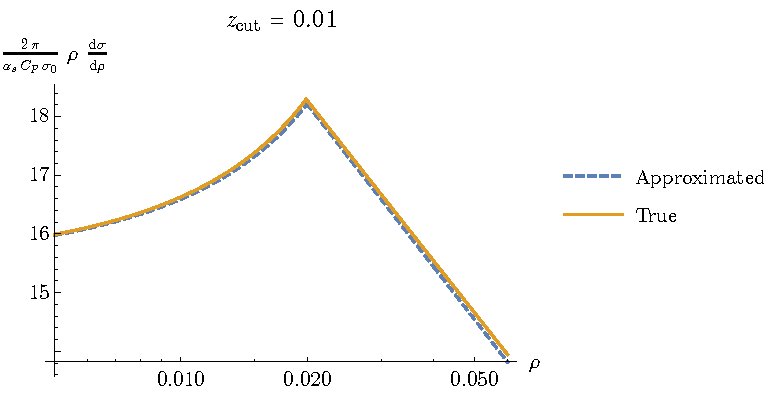
\includegraphics[width=0.9\textwidth]{figures/approximation_small_zcut_0.01.pdf}
		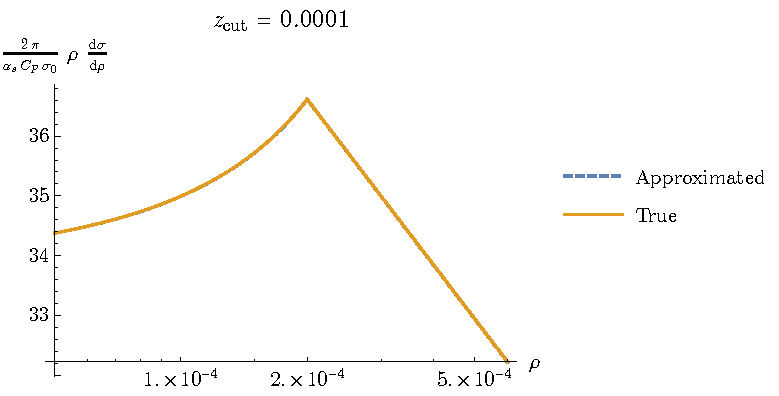
\includegraphics[width=0.9\textwidth]{figures/approximation_small_zcut_0.0001.pdf}

		\caption{\label{leading-fig:fixed order approx}True (orange solid line) and approximated (blue dashed line) distribution of groomed heavy hemisphere mass in the limit $\rho \sim \zcut \ll 1$.}
	\end{center}
	\end{figure}

	For this calculation, the true analytic distribution is known completely and can be used for comparison. From Ref.~\cite{larkoski_improving_2020}, we have
	\begin{equation}
	\begin{aligned}
		\frac{2\pi}{\alpha_s C_F}\frac{1}{\sigma_0}\frac{d\sigma}{d\rho} &= \Theta\qty(\frac{3}{4}-\rho)\Theta(\rho - (2\zcut - \zcut^2))\Bigg[ -\frac{12(6-6\sqrt{1-\rho} + \rho(-8 + 5\sqrt{1- \rho} + 2\rho))}{\rho^3(1 - \rho)} \\
		&\qquad- \frac{2(6 - 6 \sqrt{1 - \rho} - \rho(5 - 4\sqrt{1 - \rho}))}{\rho^2(1 - \rho)} \log(\frac{\rho}{2 + 2\sqrt{1 - \rho} - 3\rho}) \Bigg] \\
		&+ \Theta(2\zcut - \zcut^2 - \rho)\Bigg[ \frac{12(1 - 2\zcut)(2 - 2\sqrt{1 - \rho} - \rho)^2}{\rho^3(2 - 2\sqrt{1 - \rho} - \rho(2 - \sqrt{1 - \rho}))} \\ 
		&\hspace{-2cm}- \frac{2(6 -6 \sqrt{1 - \rho} - \rho(5 - 4\sqrt{1 - \rho}))}{\rho^2(1 - \rho)}\log(\frac{2 - 4\zcut(1 - \zcut - \sqrt{1 - \rho}) - 2\sqrt{1 - \rho} - \rho}{4\zcut(1 - \zcut) - \rho})\Bigg].
	\end{aligned}
	\end{equation}
	The true result is plotted against the approximation in Fig.~\ref{leading-fig:fixed order approx}. Notice that, as expected, the approximation gets better both as $\zcut$ becomes smaller and as $\rho$ moves closer to $\zcut$.

	Now, from the true result, we can then take the limit $\rho \sim \zcut \ll 1$ explicitly to find
	\begin{equation}
	\begin{aligned}
		\frac{2\pi}{\alpha_s C_F}\frac{1}{\sigma_0}\frac{d\sigma}{d\rho} &=\Theta(\rho - 2\zcut)\qty[-\frac{3}{\rho} + \frac{4}{\rho} \log(\frac{4}{\rho})] \\
			&\hspace{3cm}+ \Theta(2\zcut - \rho)\qty[ -\frac{3}{\rho} - \frac{4}{\rho}\log(\zcut - \frac{\rho}{4})] \\
		&= \Theta(\rho - 2\zcut)\frac{4}{\rho} \log(\frac{4}{\rho}) \\
			&\hspace{3cm}- \Theta(2\zcut - \rho)\frac{4}{\rho}\log(\zcut - \frac{\rho}{4}) - \frac{3}{\rho}.
	\end{aligned}
	\end{equation}
	Notice as well that taking the same limit in Eq.~\ref{leading-eq:fixed order result} yields
	\begin{equation}
		\frac{2\pi}{\alpha_s C_F}\frac{\rho}{\sigma_0}\frac{d\sigma}{d\rho} = 4\Theta(\rho - 2\zcut)\log(\frac{4}{\rho}) - 4\Theta(2\zcut - \rho)\log(\zcut - \frac{\rho}{4}) - 3,
	\end{equation}
	which is the same result!
	
	Thus, we see that this method works. To compute the distribution in a given limit, it suffices for us to consider only `interesting' regions of phase space, compute their contribution to the distribution, and then combine these contributions in the appropriate manner. The same principle will be applied as we work towards an all-orders calculation. 

	There, too, we will begin by identifying the singular regions of phase space and the dominant physical contributions in each region. We will need to resum the contributions in each region in order to manage the effects of imposed scales to all orders, but this is simply an additional step in the calculation. Moreover, instead of a simple sum, we will combine functions by convolving them, since we need to appropriately capture terms at every order in $\alpha_s$ hidden in each function. Despite these complications, however, the core idea is the same, and this simple example provides a general road map as we push forward.\footnote{We could think of this as a map which only contains the location of the interstate highways.}

	Finally, one should notice in the leading-order distribution the sharp cusp that occurs at $\rho = 2\zcut - \zcut^2$. It looks strange for a reason --- this cusp is entirely unphysical. It has been demonstrated that, as higher-order contributions in $\alpha_s$ are added, the cusp becomes smooth \cite{larkoski_improving_2020}. Nevertheless, this oddity should serve as a clue that there is something interesting at play. We will explore the physics further in subsequent chapters.


% \ifstandalone
% \bibliographystyle{../bsts/JHEP} 
% \bibliography{../jet_substructure}
% \fi
\end{document}
